\section{Uncertainties and Sets}
\label{uncertainties_and_sets}

As mentioned in Section~\ref{sec:robustvsstochastic}, one of the advantages
of \gls{ro} over \gls{so} is the fact that it only requires as inputs
the uncertainty set size instead of complete probability distributions
over each parameter.
In the context of this work, the set size is defined relatively in each
uncertain design parameter $u_i$ by $3\sigma_i$, and globally by scalar parameter
$\Gamma$. An illustration of the relationship between $3\sigma$'s and $\Gamma$
is provided in Figure~\ref{fig:sets}, and explained in Sections~\ref{sec:relative} and ~\ref{sec:global}.

\subsection{Design parameter uncertainties}
\label{sec:relative}

The relative size of the uncertainty set in each uncertain variable is
given by three times the \gls{cv}\footnote{The \gls{cv}
is defined as follows: $\text{CV} = \frac{\sigma}{|\mu|}$,
where $\sigma$ is the standard deviation and $\mu$ is the mean of the parameter.},
as listed in Table~\ref{tab:uncertainties}. Since for the rest of this work
all standard deviations ($\sigma$) are normalized by the means of the parameters, we will use $3\sigma$
to represent $3\text{CV}$.

\begin{table}
\begin{center}
\caption{\label{tab:uncertainties} Parameters and Uncertainties (increasing order)}
\begin{tabular}{c c c c c}
\hline
Parameters & Description & Value & \% Uncert. ($3\sigma$) \\
\hline
e & span efficiency & 0.92 & 3\\
$\mu$ & air viscosity (SL) & $1.78 \times 10^{-5}~\mathrm{kg/(ms)}$ & 4 \\
$\rho$ & air density (SL) & 1.23 $\mathrm{kg/m^3}$ & 5 \\
$C_{L,\rm{max}}$ & stall lift coefficient & 1.6 & 5\\
k & fuselage form factor & 1.17 & 10\\
$C_{f,\rm{ref}}$ & reference fuselage skin friction factor & 0.455 & 10 \\
$\rho_{\rm{p}}$ & payload density & 1.5 $\mathrm{kg/m^3}$ & 10 \\
$N_{\rm{ult}}$ & ultimate load factor & 3.3 & 15\\
$V_{\rm{min}}$ & takeoff speed & $35 \mathrm{m/s}$ & 20\\
$W_{\rm{p}}$ & payload weight & 3000 N & 20\\
$W_{\rm{coeff, strc}}$ & wing structural weight coefficient & $2 \times 10^{-5}~1/\mathrm{m}$ & 20\\
$W_{\rm{coeff,surf}}$ & wing surface weight coefficient & 60 $\mathrm{N/m^2}$ & 20\\
\hline
\end{tabular}
\end{center}
\end{table}

In this case of a conceptual aircraft design with no prior data,
the parameter uncertainties reflect aerospace engineering intuition.
The wing weight coefficients $W_{\rm{coeff, strc}}$ and $W_{\rm{coeff,surf}}$,
and the ultimate load factor $N_{\rm{ult}}$ have
large $3\sigma$'s because the build quality of aircraft components is
often difficult to quantify with a large degree of certainty.
The payload weight and density ($W_{\rm{p}}$ and $\rho_{\rm{p}}$) have large uncertainties
since the payload is often developed concurrently with the aircraft.
Parameters that engineers take to be
physical constants (sea level air viscosity and density, $\mu$ and $\rho$) and those that can be determined with
a relatively high degree of accuracy ($e$) have relatively low deviations.
Parameters that require testing to determine ($C_{L,\rm{max}}$, $C_{f,\rm{ref}}$,
$V_{\rm{min}}$) have a level of uncertainty
that reflects the expected variance of empirical studies. However, note that
these quantities are ultimately picked by the designer using prior experience and data,
and the level of conservativeness in the
design will be greatly affected by the chosen $3\sigma$'s.

\subsection{Uncertainty sets considered}
\label{sec:global}

The robust design problem is solved for box and elliptical uncertainty sets,
which are defined by the L$\infty$- and L2-norms, and bounded
by varying the parameter $\Gamma$.
Intuitively, for both sets, $\Gamma$ is a global measure of how much risk is being
hedged against, and affects all parameter uncertainties simultaneously. $\Gamma = 0$
implies that all of the parameters take their nominal values with zero uncertainty,
which we call the nominal problem,
and larger $\Gamma$ protects against greater uncertainty. $\Gamma$ is more
rigorously defined in the context of robust linear programming in~Appendix~\ref{LP_to_GP}.

\begin{figure}
    % Box uncertainty set
    \begin{subfigure}[b]{0.5\textwidth}
        \centering
        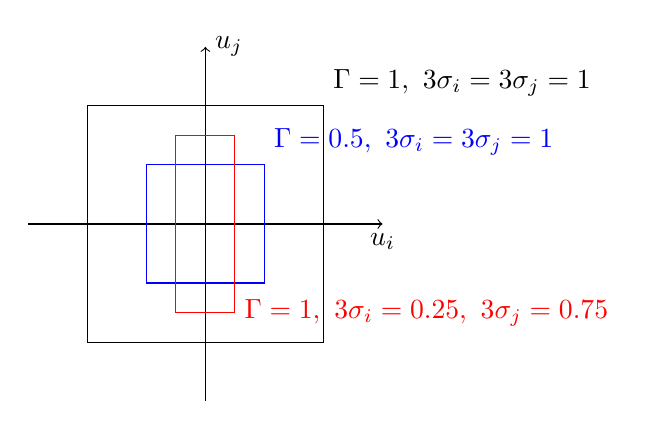
\begin{tikzpicture}[scale=1.5]
            \draw[->] (-1.5,0) -- (1.5,0) node[anchor=north] {$u_i$};
            \draw[->] (0,-1.5) -- (0,1.5) node[anchor=west] {$u_j$};
            \draw[->] (-1, -1) -- (-1, 1) -- (1, 1) node[anchor=south west] {$\Gamma=1, ~3\sigma_i = 3\sigma_j=1$} -- (1, -1) -- cycle;
            \draw[->, blue] (-0.5, -0.5) -- (-0.5, 0.5) -- (0.5, 0.5) node[anchor=south west] {\color{blue}$\Gamma=0.5, ~3\sigma_i = 3\sigma_j=1$} -- (0.5, -0.5) -- cycle;
            \draw[->, red] (-0.25, -0.75) -- (-0.25, 0.75) -- (0.25, 0.75) -- (0.25, -0.75) node[anchor=west] {\color{red}$\Gamma=1, ~3\sigma_i = 0.25, ~3\sigma_j=0.75$} -- cycle;
        \end{tikzpicture}
        \caption{Example L$\infty$ or box uncertainty sets.}
        \label{fig:setsbox}
    \end{subfigure}
    % Elliptical uncertainty set
    \begin{subfigure}[b]{0.5\textwidth}
        \centering
        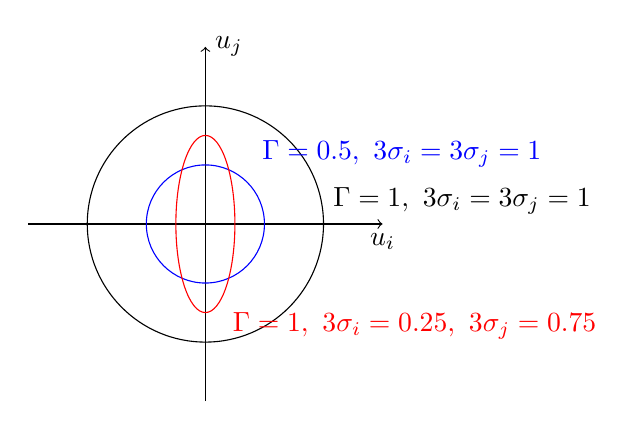
\begin{tikzpicture}[scale=1.5]
            \draw[->] (-1.5,0) -- (1.5,0) node[anchor=north] {$u_i$};
            \draw[->] (0,-1.5) -- (0,1.5) node[anchor=west] {$u_j$};
            \draw (0,0) circle (1cm);
            \node[above right] at (1.0,0) {$\Gamma=1, ~3\sigma_i = 3\sigma_j=1$};
            \draw[blue] (0,0) circle (0.5cm);
            \node [above right] at (0.4, 0.4) {\color{blue}$\Gamma=0.5, ~3\sigma_i = 3\sigma_j=1$};
            \draw[red] (0,0) ellipse (0.25cm and 0.75cm);
            \node[below right] at (0.15, -0.666) {\color{red}$\Gamma=1, ~3\sigma_i = 0.25,~3\sigma_j=0.75$};
        \end{tikzpicture}
        \caption{Example L2 or elliptical uncertainty sets.}
        \label{fig:setselliptical}
    \end{subfigure}
    \caption{$\Gamma$ defines the overall size of norm uncertainty sets, while $3\sigma$ defines the relative
    size of the set in each uncertain parameter. }
    \label{fig:sets}
\end{figure}

For box uncertainty,
$\Gamma$ scales the width of the L$\infty$ hypercube as shown in Figure~\ref{fig:setsbox},
whose dimensionality is the same as the number of uncertain parameters (12).
More intuitively, $\Gamma \times 3\sigma_i$ defines the range of the possible values of uncertain parameter $u_i$,
normalized by the mean of $u_i$.
It can be easy to assume that using margins and box uncertainty sets will yield the same designs,
but they fundamentally function differently.
Firstly, the worst case outcome in box uncertainty can come \emph{from the interior} of the uncertainty
set, instead of the corner of the hypercube considered
by margins. Furthermore, there is no guarantee (and it is unlikely)
that the chosen corner, i.e. particular allocation of margins,
is the most conservative point in the uncertainty set.
It is even possible that the \emph{the wrong sign of margin} is allocated for certain parameters,
since \gls{sp}s are nonlinear and local sensitivities cannot be used reliably to intuit global behavior. Consider
in this particular example the sea level air density $\rho$.
Higher air density is better for takeoff performance and naturally aspirated engine performance,
but results in higher drag, so it is difficult
for a designer to determine how to best allocate margin on $\rho$. Thus for the rest
of this paper the direction of margins is determined using the local sensitivities of the nominal solution,
which are obtained at no extra computational cost in the solution of the terminal \gls{gp} approximation of the \gls{sp}.
With these considerations in mind, box uncertainty is expected to be strictly more conservative
and more appropriate than the use of margins
in conceptual design, since (1) margins fail to capture the level of conservativeness they signal, and (2) prior
information (in this case the nominal solution) is required to allocate margin effectively.

For elliptical uncertainty, $\Gamma$ is the maximum diameter of the Euclidian norm
ball of $u$ as shown in Figure~\ref{fig:setselliptical},
where $u_i$ is one-third the number of standard deviations of perturbation of the
$i$th parameter from its nominal value.
Elliptical uncertainty exploits the fact that the joint probability of
multiple uncertain parameters taking values in the tails of their respective distributions is
very low. So while it does not protect deterministically for all outcomes of the uncertain
parameters within $3\sigma$, it is expected to protect against uncertain outcomes
less conservatively than the box uncertainty set, with little compromise in the
ability of the design to satisfy constraints.
